\section{Stream Programming Model Preliminaries}

%% \begin{figure}[t]
%% \begin{center}
%% %\vspace{-24pt}
%% % \framebox{
%%  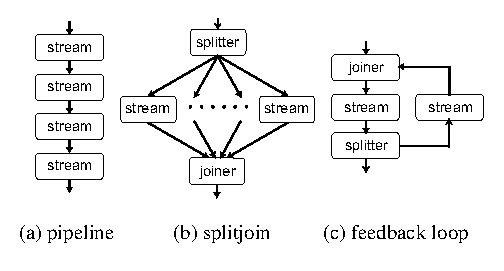
\includegraphics[scale=1, angle=0]{./constructs-eg.eps}
%% %}
%% % \vspace{-6pt}
%% % \nocaptionrule
%%  \caption{Examples of hierarchical streams.}
%%  \label{fig:containers}
%% \end{center}
%% \end{figure}

\begin{figure}[t]
\begin{center}
\psfig{figure=graph-example.eps,height=1.5in}
\vspace{9pt}
\caption{{\small Example stream graph.
\protect\label{fig:stream-rates}}}
\end{center}
\vspace{-26pt}
\end{figure}

There are are a number of stream-oriented languages drawing from
domains such as functional, dataflow, CSP and synchronous
programming~\cite{survey97}. We assume an architecture-independent
programming language for high-performance stream programming. The
language expresses computation as a graph of {\it actors} connected by
FIFO communication channels.

An execution $\phi$ of a stream program is an ordered sequence of
actor firings. Each actor follows a set of execution steps, or
phases. Each phase consumes a number of items from each input channel
and produces a number of items onto each output channel. The  ordering
of phases is known at compile time, and their execution is cyclic
(that is, after executing the last phase, the first phase is executed
again).

An example stream graph is shown in Figure~\ref{fig:stream-rates}.
Nodes are annotated with their I/O rates. For example, node $C$
consumes 3 items and produces 2 items on each execution. Node $A$ is a
round-robin splitter that produces one item on its left channel during
the first phase, and one item on its right channel during the second
phase (similarly for Node $E$).

%% We will commonly refer to actors as {\it filters} as is the case with
%% other  streaming languages,
%% e.g. StreamIt~\cite{streamitcc,streamit-lang-spec}.  Filters use
%% explicit data channels for all communication. A filter contains a {\tt
%% work} function that executes a single step of the filter.  From within
%% {\tt work}, a filter can {\it push} items onto the output channel,
%% {\it pop} items from the input channel. Some languages also allow a
%% filter to {\it peek} at an input item without removing it from the
%% channel. Peeking exposes data parallelism in sliding-window filters
%% (e.g., FIR filters). Conceptually however, it is equivalent to filters
%% that maintain some internal state that maintains the data reuse..

%% An actor is stateful if it maintains some internal state, and hence
%% requires that its phases execute sequentially. An actor is stateless
%% if it does not maintain internal state, and hence its phase executions
%% can run in parallel.

%% We assume there are three fundamental primitives for hierarchically
%% composing filters into larger stream graphs.  A {\it pipeline}
%% connects streams sequentially. A {\it splitjoin} specifies
%% independent and parallel streams that diverge from a common {\it
%% splitter} and merge into a common {\it joiner}. The final hierarchical
%% primitive is a {\it feedbackloop} that provides a way to create cycles
%% in the graph. 
%%In practice, feedbackloops are rare and we do not
%%consider them in this paper.

%%\subsection{Execution of Stream Program}

Let $\phi[i]$ denote the $i$th actor appearing in execution $\phi$.
%% and let $|\phi \wedge A|$ denote the number of times that actor $A$
%% appears in $\phi$. 
An execution is legal if the data dependencies between actors are
respected. Namely, for all $i$, the sequential firing of actor
$\phi[0]$ through $\phi[i-1]$ leaves enough items on the FIFO for
actor $\phi[i]$ to execute atomically. Let $\Phi$ denote the set of
legal executions. Note that while $\Phi$ is an infinite set, each
$\phi \in \Phi$ is a finite sequence.

\begin{figure*}[t]
\begin{center}
\vspace{-12pt}
\psfig{figure=sched-example.eps,width=5.5in}
\vspace{-4pt}
\caption{\small The stream graphs illustrate a steady
state cycle of a ``pull schedule''; execution proceeds from left to
right, and channels are annotated with the number of items present.
The second line lists the actors that fire in a pull schedule for
$E$.
\protect\label{fig:sched-example}}
\end{center}
\vspace{-12pt}
\end{figure*}

A simple example of a schedule is shown in
Figure~\ref{fig:sched-example}. It is a pull schedule for $E$. A pull
schedule is one that executes (fires) other nodes as few times as
possible for each firing of an actor $X$. This is achieved by
calculating the demand for data items on the input channels of $X$,
and then propagating the demand back through the stream graph via pull
scheduling of the actors connected to $X$. Pull scheduling results in
a fine-grained interleaving of actor firings, and executes each node
in the graph as few times as possible.

A steady state ${\cal S} \in \Phi$ is an execution that does not
change the buffering in the channels---that is, the number of items on
each channel after the execution is the same as it was before the
execution. Calculating a steady state is well-understood~\cite{LM87-i}.
The execution simulated in Figure~\ref{fig:sched-example} is a steady state,
meaning that additional entries of the pull schedule will repeat the
pattern given in the figure.

%% A data dependence between two filters $A$ and $B$ arises when there is
%% an edge between the filters in the stream graph. A simple composition
%% of the two filters into a pipeline $A\rightarrow B$ requires that $A$
%% pushes sufficient data items for $B$ to execute. We use $\rightarrow$
%% to denote a FIFO connection between two filters, such that the
%% consumer (e.g., $B$) pops data pushed into the FIFO by the producer
%% (e.g., $A$).

%% The number of data items pushed and poped (peeked) by a filter is
%% important because it allows a scheduler that orchestrates the
%% execution of the stream graph to make informed decisions that
%% typically lead to better performance. For example, if it is known to
%% the scheduler that $A$ produces two data items per work firing, and $B$
%% only consumes one item per work firing, then a scheduler can more
%% efficiently instruct a processing element that executes $B$ to run two
%% instances of $B$ for each instance of $A$.

%% A stream graph where all the filter I/O rates (i.e., push and pop
%% rates) are static is ameneable to static scheduling (i.e., at compile
%% time or at graph creating time). This has been shown in the large body
%% of work on Synchronous Dataflow (SDF)~\cite{LM87-i}, and its
%% generalization to Cyclo-Static Dataflow~\cite{BELP96}.

%% For example consider a simple pipeline consisting of three filters
%% $A\rightarrow B\rightarrow C$. Here $A\rightarrow B$ denotes a FIFO
%% connection between filters $A$ and $B$ such that $B$ pops data pushed
%% by $A$; and similarly for $B\rightarrow C$. A pull schedule for $C$ is
%% one that executes (fires) other nodes as few times as possible for
%% each firing of $C$. This is achieved by calculating the demand for
%% data items on the input channels of $C$, and then propagating the
%% demand back through the stream graph via pull scheduling of the
%% filters connected to $C$. Pull scheduling results in a fine-grained
%% interleaving of filter firings, and executes each node in the graph as
%% few times as possible for $C$ to fire a desired number of times.
%% Assuming that $A$ pushes two items and $B$ pops and pushes one item
%% per work firing, the pull schedule for one $C$ firing requires one
%% firing of $A$ followed by one firing of $B$. The schedule for two
%% firings of $C$ requires one firing of $A$ and two firings of $B$.
%% Note that the following two schedules execute $C$ twice: $(ABBCC)$
%% and $(ABCBC)$.
